\documentclass{article}

\usepackage[preprint]{neurips_2026}

\usepackage[utf8]{inputenc}
\usepackage[T1]{fontenc}
\usepackage{hyperref}
\usepackage{url}
\usepackage{booktabs}
\usepackage{amsfonts}
\usepackage{amsmath}
\usepackage{amsthm}
\newtheorem{proposition}{Proposition}
\usepackage{microtype}
\usepackage{xcolor}
\usepackage[english]{babel}
\usepackage{subcaption}
\usepackage{graphicx}
\usepackage{multirow}
\usepackage{siunitx}
\usepackage{float}
\usepackage{algorithm}
\usepackage{algpseudocode}
\usepackage[nameinlink]{cleveref}

\newcommand{\TODO}[1]{\textcolor{red}{TODO: #1}}

\title{Continuous Time Reinforcement Learning in Finance}

\author{%
  Hugo Belzil \\
  \And
  Leandro Bentele \\
  \And
  Fynn Starke \\
  \And
  Álvaro Zamanillo \\
}

\begin{document}

\maketitle


\begin{abstract}
This paper evaluates the differential Temporal Difference (dTD) framework of \citet{settai2025}, a model-free reinforcement learning method that targets the Hamilton-Jacobi-Bellman (HJB) equation in continuous time, and tests its viability in financial stochastic optimal control. We first replicate the benchmarks of \citet{settai2025} on continuous control tasks, confirming that the hybrid $\beta$-dTD scheme improves the policy faster than standard TD early in training. We then apply it to a genuine stochastic control problem, the continuous-time Merton consumption-investment problem, where pure dTD fails in diffusion-heavy regimes: as the observation interval $\Delta t \to 0$, the dTD gradient is dominated by the Brownian increments, and the value function collapses to a constant ($\nabla V \to 0$). We study two ways to counter this, the hybrid $\beta$-dTD regularizer and a multi-sample ($K$-sample) drift estimator. The $K$-sample estimator restores convergence in the infinite-horizon setting but is computationally expensive, whereas a finite-horizon formulation regularizes the problem more naturally and lets $\beta$-dTD outperform standard TD under low process noise. Overall, our results show both the appeal of HJB-based reinforcement learning and the difficulty of applying it under financial-scale diffusion.
\end{abstract}


\section{Introduction}
\label{sec:introduction}

Deep reinforcement learning has become a powerful paradigm for sequential decision-making, from board games to robotic control. Yet a persistent gap remains between discrete-time algorithms and systems that are naturally continuous in both state and time---physical systems, autonomous driving, and high-frequency financial markets, whose dynamics are best described by stochastic differential equations (SDEs).

When standard deep RL algorithms (e.g.\ PPO or DDPG) are applied to such environments, they first discretize time into a fixed interval $\Delta t$ and treat the problem as a Markov decision process whose value function depends on the transition kernel $P(s_{t+\Delta t} \mid s_t, a_t)$. Approximating this expectation from sampled pairs $(s_t, s_{t+\Delta t})$ discards the structural prior of temporal and spatial continuity: the updates never see the smooth trajectory connecting the two states. \citet{settai2025} identify this shortcoming and propose a remedy.

Stochastic optimal control offers an alternative. There, Bellman's principle of optimality takes the form of the Hamilton-Jacobi-Bellman (HJB) equation, which---unlike the standard Bellman equation---retains continuity explicitly through infinitesimal drift and diffusion coefficients. Classically, exploiting this required model-based knowledge of the drift $\mu$ and diffusion $\sigma$, a restrictive assumption in quantitative finance and economics, where the dynamics are latent, noisy, and non-stationary.

The Differential Temporal Difference (dTD) framework of \citet{settai2025} removes this requirement by replacing $\mu$ and $\sigma$ with sample-based finite-difference estimators of the observed increments $\Delta s_t$, yielding a model-free method that targets the fixed-policy HJB equation directly. It is data-efficient on drift-governed robotic benchmarks, but its behavior in noise-dominated regimes is untested: unlike physical systems, financial assets carry far more diffusion than drift.

Our contributions are threefold. First, we replicate the dTD benchmarks on standard continuous control tasks (Hopper, HalfCheetah, Ant, and Humanoid) using a $\beta$-dTD hybrid scheme. Second, extending the framework to the classic continuous-time Merton consumption-investment problem, we expose and explain a failure mode absent from the original drift-dominated benchmarks: as $\Delta t \to 0$ the first-order gradient estimator becomes dominated by Brownian noise, driving the critic toward a spurious constant attractor ($\nabla V \to 0$), which we make precise in \cref{prop:noise}. Third, we study two remedies---multi-sample ($K$-sample) variance reduction and a finite-horizon formulation---and characterize when each restores stable learning.

\section{Theoretical Framework}
\label{sec:theoretical_framework}

\subsection{Problem Setting}
We consider a continuous-time reinforcement learning setup where the system state space is defined as $\mathcal{S} \subset \mathbb{R}^n$ and the action space as $\mathcal{A}$. The infinitesimal evolution of the state trajectory is governed by a controlled Stochastic Differential Equation of the form:
\begin{equation}
    dS_t = \mu(S_t, A_t) dt + \sigma(S_t, A_t) dB_t
\end{equation}
where $\mu: \mathcal{S} \times \mathcal{A} \to \mathbb{R}^n$ denotes the drift coefficient, $\sigma: \mathcal{S} \times \mathcal{A} \to \mathbb{R}^{n \times m}$ represents the diffusion matrix, and $(B_t)_{t \ge 0}$ is an $m$-dimensional standard Brownian motion. Actions are sampled according to a stationary stochastic policy $A_t \sim \pi(\cdot | S_t)$. The model-free assumption dictates that the agent has no \textit{a priori} knowledge of the analytical forms of $\mu$ or $\sigma$, observing the system states exclusively at discrete temporal instants $t, t+\Delta t, t+2\Delta t, \dots$.

\subsection{Classical Temporal Difference (TD) Learning Baseline}
Before establishing the continuous-time framework, we review the classical discrete-time Temporal Difference (TD) learning paradigm, which serves as our fundamental baseline. In a standard Markov Decision Process (MDP) setting, time is treated as a sequence of discrete steps, and an agent's goal is to evaluate a policy $\pi$ by learning its expected discounted cumulative return, defined as the value function $V^\pi(s)$:
\begin{equation}
    V^{\pi}(s) = \mathbb{E}_{\pi} \left[ \sum_{k=0}^{\infty} \gamma_{\text{discrete}}^{k} r(s_k, a_k) \;\middle|\; s_0 = s \right]
\end{equation}
where $\gamma_{\text{discrete}} \in (0, 1)$ represents the discrete discount factor and $r(s_k, a_k)$ is the immediate reward observed after executing action $a_k \sim \pi(\cdot|s_k)$ from state $s_k$. This formulation satisfies the classic discrete-time \textbf{Bellman expectation equation}:
\begin{equation}
    V^{\pi}(s) = \mathbb{E}_{a \sim \pi(\cdot|s), \, s' \sim P(\cdot|s,a)} \left[ r(s, a) + \gamma_{\text{discrete}} V^{\pi}(s') \right]
\end{equation}
where $P(\cdot|s,a)$ denotes the transition kernel of the environment conditioned on the current state-action pair, and the action is sampled according to the stationary policy $\pi(\cdot|s)$.

In an online, model-free setting, the true transition dynamics $P^\pi$ are unknown. Standard TD learning (specifically TD(0)) approximates this expectation by utilizing sampled transitions $(s_t, a_t, r_t, s_{t+1})$ directly from execution paths. Let $V_\theta(s)$ represent the estimated value function parameterized by a neural network with weights $\theta$. Upon observing a transition, the algorithm evaluates the prediction error via the \textbf{TD error ($\delta_t$)}:
\begin{equation}
    \delta_t = r_t + \gamma_{\text{discrete}} V_{\bar{\theta}}(s_{t+1}) - V_{\theta}(s_t)
\end{equation}
where $\bar{\theta}$ denotes a detached, frozen copy of the network parameters used to compute the bootstrap target to maintain training stability. The corresponding network value loss optimized via gradient descent is defined as:
\begin{equation}
    \mathcal{L}_{\text{TD}}(\theta) = \frac{1}{2} \mathbb{E} \left[ \delta_t^2 \right]
\end{equation}

While this formulation underpins most state-of-the-art discrete reinforcement learning algorithms, it exhibits a structural flaw when dealing with underlying continuous-time setups. Because the value function update only evaluates discrete, disjoint state-action pairs $(s_t, s_{t+1})$, the sampling mechanism skips over all intermediate spatial states traversed during the observation window, disregarding continuity information.

% Actor-Critic background --- omitted from the rendered paper. Not load-bearing:
% the policy is fixed at the analytical optimum in all experiments (only the critic
% is learned), and nothing references this subsection. Kept here for reference.
%
% \subsection{The Actor-Critic Optimization Paradigm}
% While the classical TD learning framework outlines how to evaluate a value function under a fixed policy, modern continuous control reinforcement learning algorithms - such as Proximal Policy Optimization (PPO) - must simultaneously optimize the underlying policy to maximize expected returns. This is naturally operationalized via the Actor-Critic architecture. This framework splits the decision-making and evaluation tasks between two specialized neural network function approximators:
%
% \begin{enumerate}
%     \item \textbf{The Actor (Policy Network):} Parameterized by weights $\phi$, the actor represents the stochastic policy $\pi_\phi(a|s)$. Its objective is to propose optimal actions in a given state to maximize the long-term expected discounted return.
%     \item \textbf{The Critic (Value Network):} Parameterized by weights $\theta$, the critic represents the value function $V_\theta(s)$. It scores the expected utility of the states visited under the actor's current policy by minimizing the mean-squared temporal difference error $\delta_t$.
% \end{enumerate}
%
% During online execution, the calculated temporal difference error $\delta_t$ plays a dual role in driving joint parameter optimization. The critic uses the squared residual to update its value-matching landscape. Concurrently, the error serves as an unbiased advantage signal to update the actor:
% \begin{itemize}
%     \item If $\delta_t > 0$, the realized transition yielded a higher return than expected by the critic's  baseline; the actor's policy gradient update scales to increase the log-probability of that action under the current state.
%     \item If $\delta_t < 0$, the chosen action underperformed relative to expectation, and the actor updates to diminish its selection probability.
% \end{itemize}
%
% This synchronized feedback loop establishes the baseline control framework. In the subsequent sections, we transition to a continuous-time optimal control perspective to show how this baseline can be regularized by substituting discrete pairs $(s_t, s_{t+\Delta t})$ with infinitesimal spatial derivatives derived from the environment's underlying stochastic differential equation.

\subsection{The HJB Equation under a Fixed Policy}
For a fixed policy $\pi$, our objective is to learn the value function $V^\pi(s)$, representing the expected discounted cumulative reward rate $\rho(s, a)$ over an infinite horizon:
\begin{equation}
    V^\pi(s) = \mathbb{E}_{p_\pi} \left[ \int_0^\infty e^{-\gamma t} \rho(S_t, A_t) dt \;\middle|\; S_0 = s \right]
\end{equation}
where $\gamma > 0$ is the continuous discount rate. In a discretized framework with an observation interval $\Delta t$, this satisfies the discrete-time Bellman expectation equation:
\begin{equation}
    V^\pi(s_t) = \mathbb{E}_{p_\pi} \left[ \rho(s_t, A_t)\Delta t + e^{-\gamma \Delta t} V^\pi(S_{t+\Delta t}) \right]
\end{equation}
Assuming that $V^\pi$ is at least $C^2$, we can expand the term $V^\pi(S_{t+\Delta t})$ using It\^o's formula:
\begin{align}
    V^\pi(S_{t+\Delta t}) &= V^\pi(s_t) + \left( \sum_{i=1}^n \mu^i(s_t, A_t) \frac{\partial V^\pi(s)}{\partial s^i}\Big|_{s_t} \right.\nonumber\\
    &\quad \left. + \frac{1}{2} \sum_{i=1}^n \sum_{j=1}^n \left[\sigma(s_t, A_t)\sigma^\top(s_t, A_t)\right]^{ij} \frac{\partial^2 V^\pi(s)}{\partial s^i \partial s^j}\Big|_{s_t} \right) \Delta t \nonumber\\
    &\quad + \sum_{i=1}^n \sum_{j=1}^m \sigma_j^i(s_t, A_t)\frac{\partial V^\pi(s)}{\partial s^i}\Big|_{s_t} (B^j_{t+\Delta t} - B^j_t) + O(\Delta t^{3/2})
\end{align}
Taking the expectation $\mathbb{E}_{p_\pi}[\cdot]$, the martingale property eliminates the Brownian motion increment since $\mathbb{E}[B^j_{t+\Delta t} - B^j_t] = 0$. Approximating $e^{-\gamma \Delta t} \approx 1 - \gamma \Delta t$, substituting the expansion back into the Bellman equation, dividing by $\Delta t$, and evaluating the continuous limit as $\Delta t \to 0$ yields the Hamilton-Jacobi-Bellman (HJB) equation for a fixed policy:
\begin{equation}
    V^\pi(s_t) = \frac{1}{\gamma} \mathbb{E}_{\pi} \left[ \rho(s_t, A_t) + \sum_{i=1}^n \mu^i(s_t, A_t) \frac{\partial V^\pi(s)}{\partial s^i}\Big|_{s_t} + \frac{1}{2} \sum_{i=1}^n \sum_{j=1}^n [\sigma\sigma^\top]^{ij} \frac{\partial^2 V^\pi(s)}{\partial s^i \partial s^j}\Big|_{s_t} \right]
\end{equation}

\subsection{Model-Free Derivation of dTD}
Direct sample-based evaluation of the HJB expectation equation is traditionally impossible without modeling $\mu$ and $\sigma$. To circumvent this limitation, \citet{settai2025} prove that the drift and diffusion coefficients can be replaced by taking the limits of sample-based finite differences of the state increments:
\begin{align}
    \mathbb{E}_{\pi}[\mu^i(s_t, A_t)] &= \lim_{\Delta t \to 0} \mathbb{E}_{p_\pi} \left[ \frac{S^i_{t+\Delta t} - s^i_t}{\Delta t} \right] \\
    \mathbb{E}_{\pi}[[\sigma(s_t, A_t)\sigma^\top(s_t, A_t)]^{ij}] &= \lim_{\Delta t \to 0} \mathbb{E}_{p_\pi} \left[ \frac{(S^i_{t+\Delta t} - s^i_t)(S^j_{t+\Delta t} - s^j_t)}{\Delta t} \right]
\end{align}
Substituting these finite-difference estimators into the fixed-policy HJB equation yields a model-free continuous-time residual operator. Let $\hat{V}$ represent an estimated value function parameterized by a neural network and define $\Delta s_t = s_{t+\Delta t} - s_t$. The differential temporal difference (dTD) residual is given by:
\begin{equation}
    \label{eq:residual}
    dTD := \frac{1}{\gamma} \left( \rho(s_t, a_t) + \frac{1}{\Delta t}\Delta s_t^\top \nabla \hat{V}(s_t) + \frac{1}{2\Delta t} \Delta s_t^\top \nabla^2 \hat{V}(s_t) \Delta s_t \right) - \hat{V}(s_t)
\end{equation}

\subsection{Method Overview}
\subsubsection{From TD to dTD}
The classic, well-established TD will serve as a performance benchmark. When incorporating the dTD residual into a gradient descent framework, the architectural division between the target (detached teacher) and prediction (gradient-receiving student) is not unique according to \citet{settai2025}. While \textit{naive-dTD} maintains the traditional layout where the standalone value function $\gamma V(s_t)$ acts as the prediction, the refined \textit{dTD} scheme maps the spatial gradients and Hessians to the prediction term. This forces gradient descent to directly optimize the smoothness and geometry of the critic network rather than merely performing value-matching. It is worth highlighting that the prediction parameters receive active gradient updates, while the bootstrap target is detached to remain constant during the optimization step.

\begin{table}[htbp]
\centering
\caption{Comparison of Target and Prediction terms across different TD formulations.}
\label{tab:td_methods}
\resizebox{\textwidth}{!}{%
\begin{tabular}{lll}
\toprule
\textbf{Method} & \textbf{Target (Fixed / Detached)} & \textbf{Prediction (Active Gradients)} \\ \midrule
\textbf{Standard TD} & $r(s_t, a_t) + \gamma_{\text{discrete}} V(s_{t+1})$ & $V(s_t)$ \\ \addlinespace
\textbf{naive-dTD} & $\rho(s_t, a_t) + \frac{\Delta s_t}{\Delta t} \cdot \nabla V + \frac{1}{2\Delta t} \Delta s_t^\top \nabla^2 V \Delta s_t$ & $\gamma V(s_t)$ \\ \addlinespace
\textbf{dTD} & $-\rho(s_t, a_t) + \gamma V(s_{t+\Delta t})$ & $\frac{\Delta s_t}{\Delta t} \cdot \nabla V + \frac{1}{2\Delta t} \Delta s_t^\top \nabla^2 V \Delta s_t$ \\ \bottomrule
\end{tabular}%
}
\end{table}

\subsubsection{\texorpdfstring{$\beta$}{beta}-dTD Stabilization Scheme}
While the pure dTD formulation possesses elegant continuous-time convergence properties in an idealized infinite-dimensional functional space, implementing it with non-linear neural network function approximators introduces significant practical instabilities. In empirical settings, function approximation errors and optimization noise can cause plain dTD updates to diverge or become trapped in spurious attractors.

To regularize the training dynamics and provide empirical robustness, \citet{settai2025} introduced a hybrid objective framework termed $\beta$-dTD. This scheme forms a linear combination of the classical discrete-time temporal difference loss and the continuous-time dTD loss using a mixture parameter $\beta \in [0, 1]$. Let $\mathcal{L}_{\text{TD}}(\theta)$ define the standard mean-squared Bellman error loss and $\mathcal{L}_{\text{dTD}}(\theta)$ represent the mean-squared differential error loss over a mini-batch of sampled transitions $\mathcal{D}$:
\begin{align}
    \mathcal{L}_{\text{TD}}(\theta) &= \frac{1}{|\mathcal{D}|} \sum_{d \in \mathcal{D}} \left( \left[ r(s_t^d, a_t^d) + \gamma_{\text{discrete}} V_{\bar{\theta}}(s_{t+\Delta t}^d) \right] - V_\theta(s_t^d) \right)^2 \\
    \mathcal{L}_{\text{dTD}}(\theta) &= \frac{1}{|\mathcal{D}|} \sum_{d \in \mathcal{D}} \left( y_d - \left[ \frac{\Delta s_t^d}{\Delta t} \cdot \nabla V_\theta(s_t^d) + \frac{1}{2\Delta t} (\Delta s_t^d)^\top \nabla^2 V_\theta(s_t^d) \Delta s_t^d \right] \right)^2
\end{align}
where $\bar{\theta}$ denotes the detached target network parameters and $y_d = -\rho(s_t^d, a_t^d) + \gamma V_{\bar{\theta}}(s_{t+\Delta t}^d)$ represents the detached dTD target. The complete $\beta$-dTD optimization objective is formulated as:
\begin{equation}
    \mathcal{L}_{\beta\text{-dTD}}(\theta) = (1 - \beta) \mathcal{L}_{\text{TD}}(\theta) + \beta \mathcal{L}_{\text{dTD}}(\theta)
\end{equation}

By parameterizing the update rule this way, the standard discrete TD component acts as a stabilizing anchor that ensures global convergence, while the dTD term injects information of continuity via spatial gradient and Hessian trajectory geometry directly into the network updates. Setting $\beta = 0$ perfectly recovers the standard discrete-time TD algorithm, whereas $\beta = 1$ simplifies to the pure model-free HJB differential update.

\section{Replication of Benchmark Results}
\label{sec:replication}

\subsection{Experimental Setup and Hyperparameters}
To validate the empirical claims of \citet{settai2025}, we first replicated the continuous control benchmarks using the Brax physics engine across four distinct high-dimensional environments: Hopper ($11$ dimensions), HalfCheetah ($17$ dimensions), Ant ($27$ dimensions), and Humanoid ($244$ dimensions). Following the paper's experimental protocol, we evaluated the algorithms under three discrete observation noise coefficients ($\text{coeff} \in \{0.00, 0.01, 0.05\}$). It is worth mentioning that the dynamics for this experiment are not an SDE; they are fully deterministic. Randomness only occurs in the observation of the state:
\begin{equation}
    s_i \leftarrow s_i + \text{coeff} \times |s_i| \times \epsilon, \quad \epsilon \sim \mathcal{N}(0, 1)
\end{equation}
The optimal mixture ratios identified for $\beta$-dTD were $\beta = 0.572$ for Hopper, $\beta = 0.742$ for HalfCheetah, $\beta = 0.241$ for Ant, and $\beta = 0.332$ for Humanoid, so the tuned $\beta$ for $\beta$-dTD is non-negligible.

\subsection{Comparative Analysis and Discussion}
As demonstrated in \cref{fig:replication_comparison}, our replicated training trajectories for most environments closely match the findings reported by \citet{settai2025} (whose original results are reproduced in \cref{fig:paper_res} of the appendix). However, for the high-dimensional Humanoid environment, we observe highly unstable and volatile training dynamics. This optimization divergence is likely driven by the severe dimensionality challenges inherent to tracking second-order spatial derivatives over a 244-dimensional state space.

\begin{figure}[t]
    \centering
    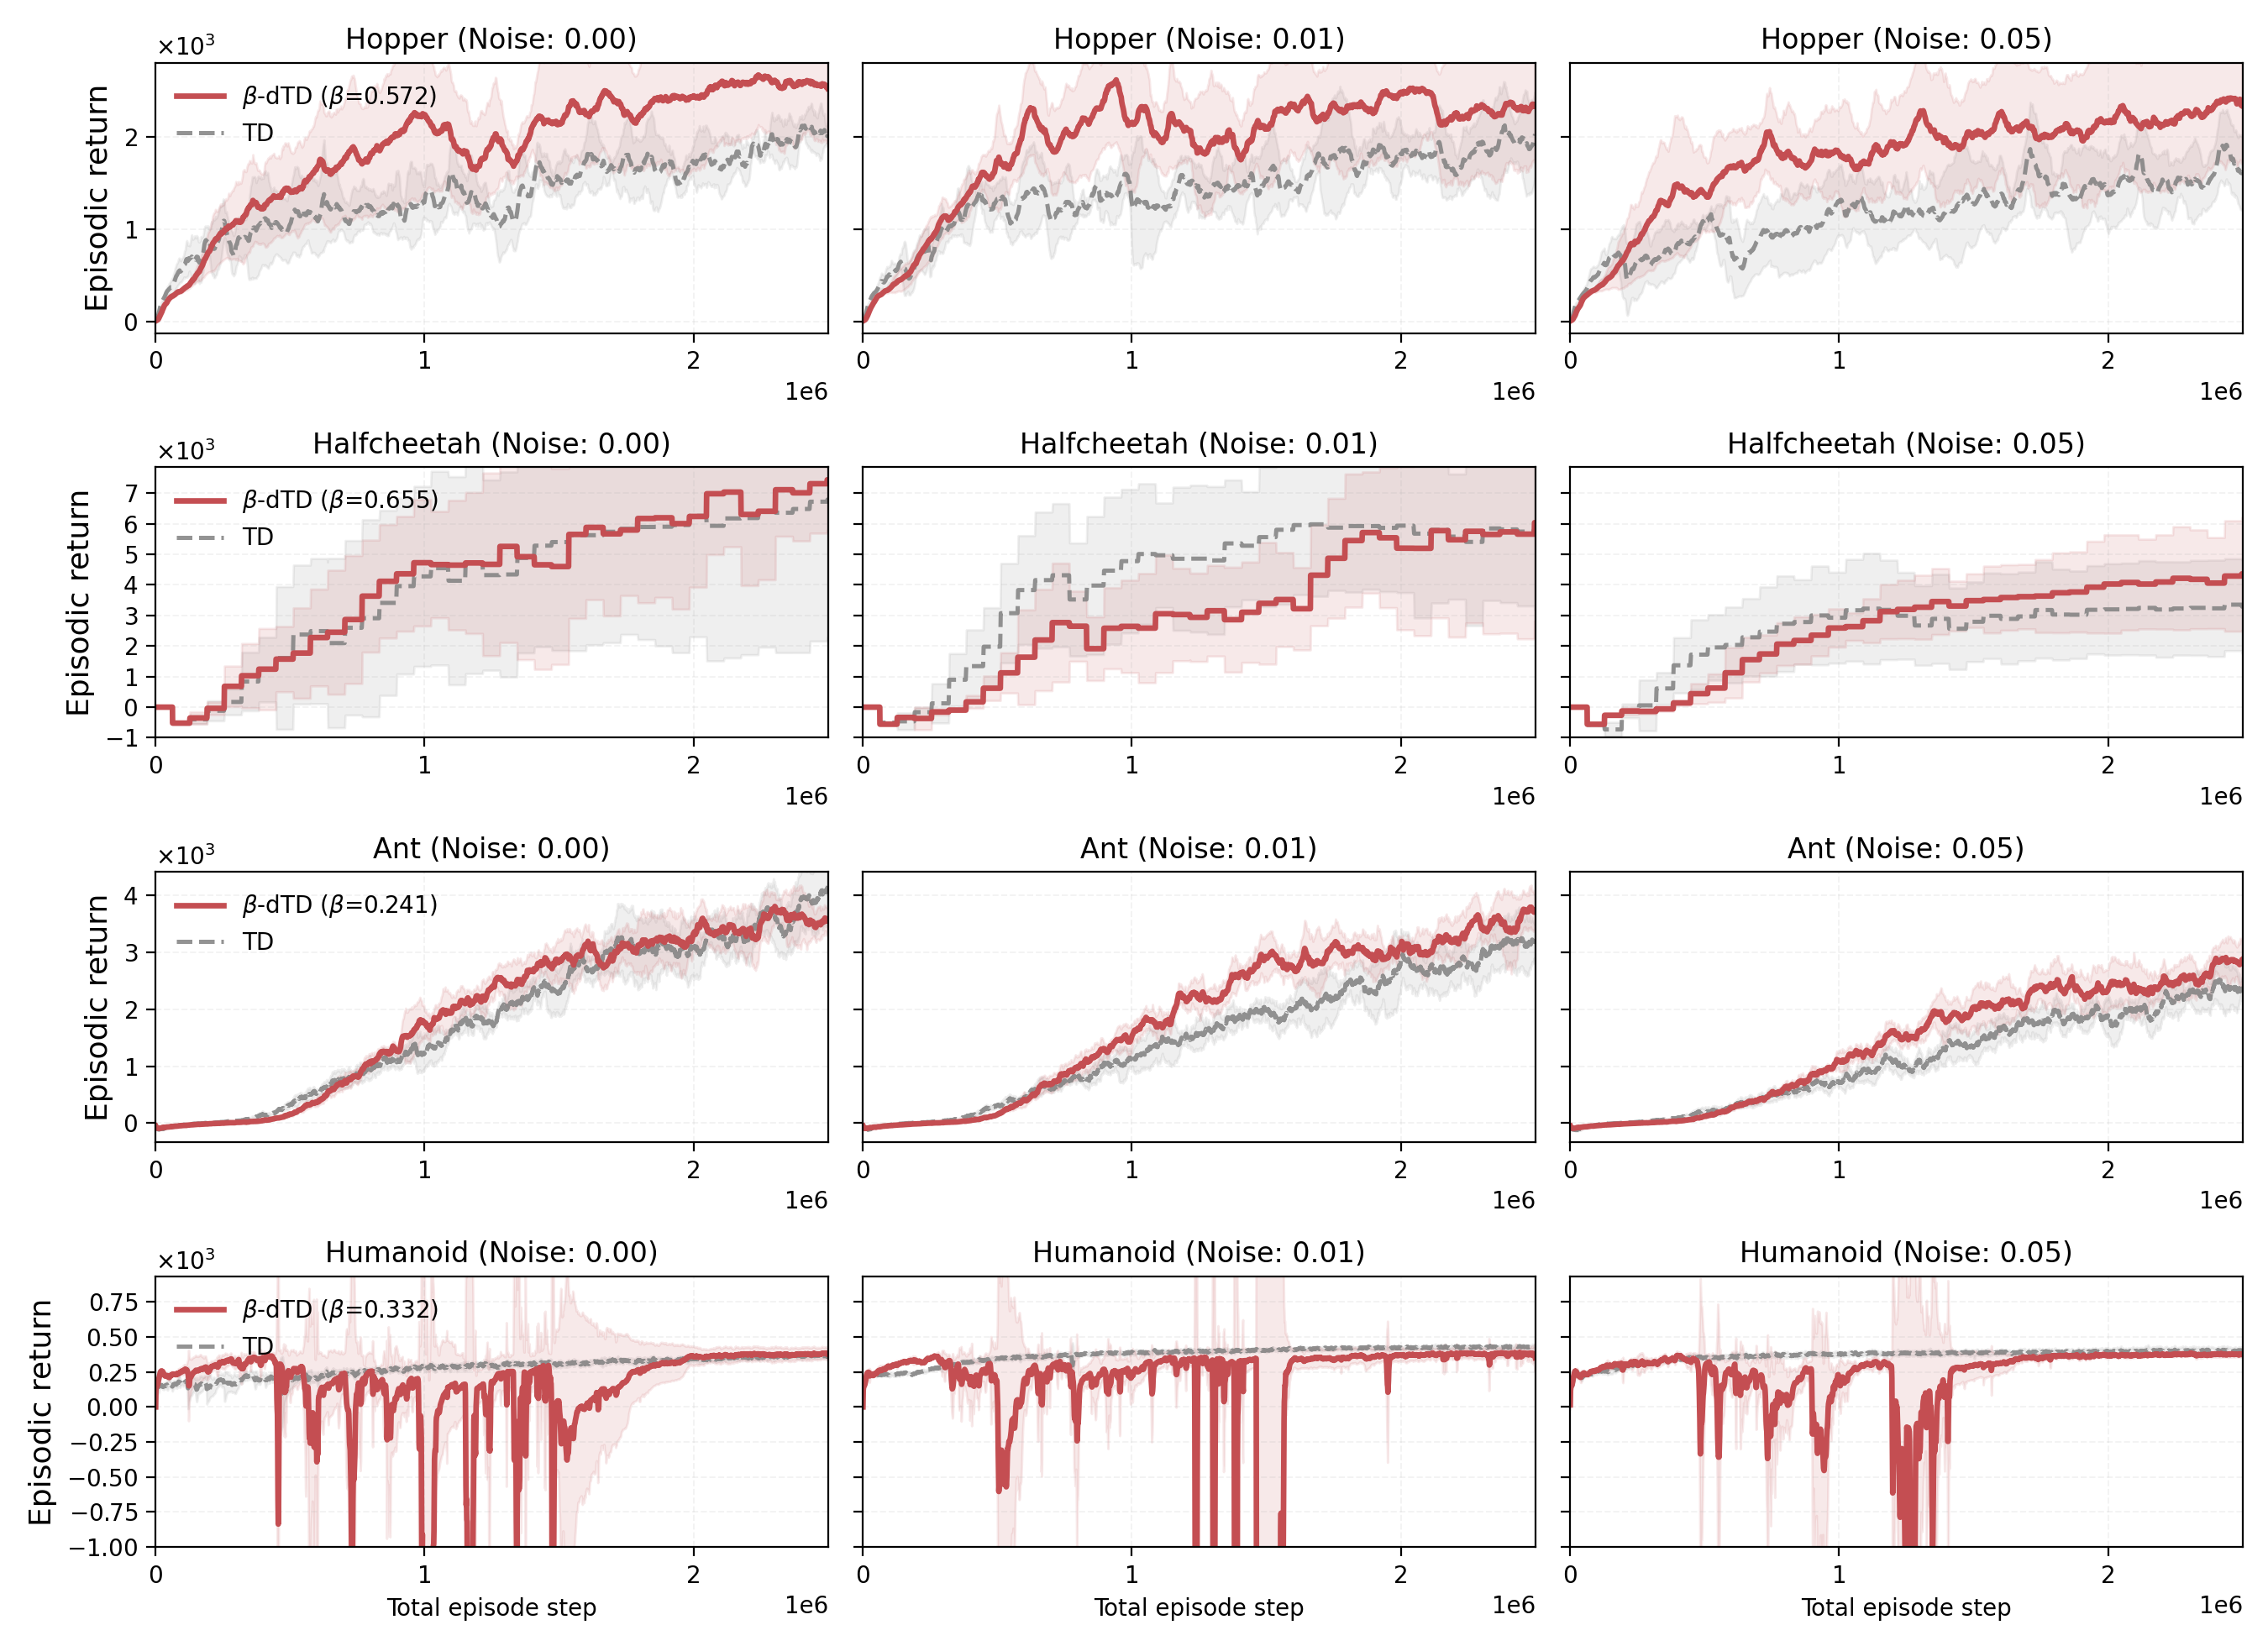
\includegraphics[width=\textwidth,height=0.34\textheight,keepaspectratio]{media/all_envs_average.png}
    \caption{Replicated episodic learning trajectories on the Brax benchmarks across observation-noise profiles ($\text{coeff} \in \{0.00, 0.01, 0.05\}$): $\beta$-dTD (red) versus standard TD (grey). The corresponding original results of \citet{settai2025} are reproduced in \cref{fig:paper_res} for comparison.}
    \label{fig:replication_comparison}
\end{figure}
Two critical insights emerge from the benchmarking phase:
\begin{enumerate}
    \item \textbf{Failure of \textit{naive-dTD}:} In line with the paper's findings, the tuned value of $\beta$ for $\beta$-naive-dTD consistently collapsed toward $0$, approximating standard TD updates yet yielding structurally sub-optimal performance. This highlights that parameterizing the standalone function $\gamma V(s_t)$ as the gradient prediction target disrupts the training topology of neural network function approximators.
    \item \textbf{Acceleration Properties of \textit{dTD}:} Conversely, $\beta$-dTD maintains a highly meaningful impact throughout the learning process because the optimized $\beta$ values remain large (notably $\beta = 0.742$ in HalfCheetah). While both standard TD and $\beta$-dTD eventually converge to similar asymptotic return boundaries due to sharing the underlying Bellman expectation target, $\beta$-dTD leverages spatial trajectory continuity to demonstrate a superior rate of policy improvement during early training stages.
\end{enumerate}

\section{Extension to the Merton Consumption-Investment Problem}
\label{sec:merton}
As mentioned in the previous section, one major weakness of the experiments selected to test the dTD method is that they were not truly SDE-driven systems. To address this, we now consider a genuine SDE problem: the Merton consumption-investment problem.

The Merton problem consists of maximizing the utility derived from consumption. To this end, we consider a wealth process $W_t$ with the following dynamics\footnote{The notation in this section is changed slightly to remain consistent with Merton's original notation. In particular, $\gamma$ now denotes the risk-aversion coefficient, $\rho$ the discount rate, and $r$ the risk-free rate.}:

\begin{equation}
\frac{d W_t}{W_t} = \big(r + \pi_t(\mu_{BS}-r) - \kappa_t\big)\,dt + \pi_t\,\sigma_{BS}\,dB_t,
\qquad c_t = \kappa_t W_t,
\end{equation}

where $r$ is the risk-free rate, $\mu_{BS}$ the expected return of the risky asset, $\sigma_{BS}$ its volatility, $\pi_t$ the fraction of wealth invested in the risky asset, and $\kappa_t$ the fraction of wealth consumed. The objective is to maximize the expected discounted utility of consumption:

\begin{equation}\label{Merton-cost}
\mathbb{E}\!\left[\int_0^\infty e^{-\rho t}\, U(c_t)\,dt\right],
\qquad U(c)=\frac{c^{1-\gamma}}{1-\gamma}, \quad \gamma > 0,\ \gamma \neq 1.
\end{equation}

For this choice of utility function, there is a closed-form solution \citep{merton1971optimum}. This is extremely useful, as it allows us to directly assess the quality of the learned value function, rather than relying on the evolution of the reward over training, as was necessary in the Brax experiments (where no closed-form solution exists).

Concretely, for this constant relative risk aversion (CRRA) specification, the optimal constant policy is
\begin{equation}\label{eq:sol_Merton}
     \pi^* = \frac{\mu_{BS}-r}{\gamma\sigma_{BS}^2},
        \qquad
        \kappa^* = \frac{\rho-(1-\gamma)\left(r + \frac{1}{2}\frac{(\mu_{BS}-r)^2}{\gamma\sigma_{BS}^2}\right)}{\gamma}.
\end{equation}

Note that the controls in \cref{eq:sol_Merton} are constant: although the wealth invested in the risky asset and the wealth consumed vary over time, their respective \emph{fractions} of total wealth remain fixed. Under any constant policy $(\pi,\kappa)$, the value function also admits a closed form,
\begin{equation}\label{eq:value_Merton}
     V^{\pi,\kappa}(w)=A(\pi,\kappa)\,\frac{w^{1-\gamma}}{1-\gamma},
     \qquad
      A(\pi,\kappa)=
            \frac{\kappa^{1-\gamma}}
            {\rho-(1-\gamma)\!\left[r+\pi(\mu_{BS}-r)-\kappa-\tfrac{1}{2}\gamma\pi^2\sigma_{BS}^2\right]},
\end{equation}
which is finite provided the denominator of $A(\pi,\kappa)$ is strictly positive. This is the expression we use as ground truth when computing the mean-absolute error (MAE) of the learned critic.

To isolate the behavior of the dTD loss, we fix the actor at the analytical optimal policy $(\pi^*,\kappa^*)$ and learn only the critic, i.e.\ the corresponding optimal value function, via gradient descent on the dTD loss or one of its variants. Fixing the policy removes confounding effects from policy optimization and lets us measure the learned value function directly against the closed-form ground truth. This procedure is summarized in \cref{pseudo:dtd}.

\begin{algorithm}[H]
        \caption{Infinite-Horizon dTD Learning}
        \begin{algorithmic}[1]

        \State \textbf{Initialize} critic parameters $\theta$ and initial states $w_0$

        \For{each iteration}
            \State Sample transitions $(w_t, w_{t+\Delta t}, r_t)$ under the fixed policy $(\pi^*,\kappa^*)$
            \State Compute the dTD loss $\mathcal{L}(\theta)$
            \State Update $\theta$ via gradient descent on $\mathcal{L}$
            \State $w_t \leftarrow w_{t+\Delta t}$
        \EndFor
        \label{pseudo:dtd}

        \end{algorithmic}
\end{algorithm}

Unless otherwise stated, the following experiments use $\mu_{BS}=0.08$, $\sigma_{BS}=0.2$, $r=0.02$, $\Delta t = 1/252$, $\gamma=2$, and $\rho=0.08$.

When pure dTD is used as the loss for learning the value function, the neural network parametrizing $V$ collapses to a constant, as shown in \cref{fig:collapse}. This collapse persists even when the network is pre-trained using the closed-form expression for the optimal value function (see \cref{fig:pretrained}).

\begin{figure}[h]
    \centering
    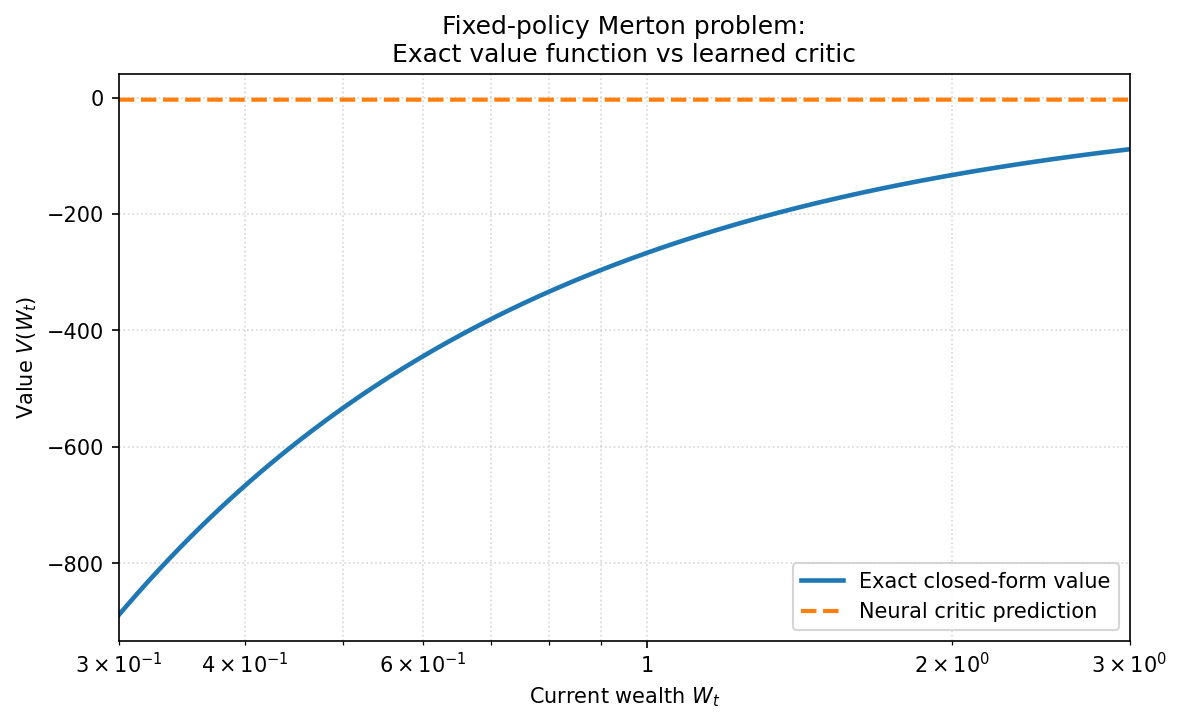
\includegraphics[width=0.5\linewidth]{media/dtd_value_fit.png}
    \caption{Value function learned with the pure dTD loss collapses to a constant}
    \label{fig:collapse}
\end{figure}

The cause of this behavior was briefly presented earlier: the drift estimator in the dTD residual (\cref{eq:residual}) is asymptotically unbiased but highly noisy. The prediction term in the loss is
$$\text{pred} = \frac{\Delta s}{\Delta t}\,\nabla V(s_t) + \frac{1}{2}\frac{(\Delta s)^2}{\Delta t}\,\nabla^2 V(s_t),$$
and its noise is characterized by the following observation.

\begin{proposition}[Diffusion-driven blow-up of the dTD estimator\footnote{The same intuition underlies a result of \citet{jiazhou2022}: in continuous time, minimizing the mean-square TD error is inconsistent because it is asymptotically equivalent to minimizing the quadratic variation $\tfrac{1}{\Delta t}\langle M \rangle_T = \tfrac{1}{\Delta t}\int_0^T \|\sigma\,\nabla V\|^2\,\mathrm{d}t$ of the value martingale $M$, whose minimizer is again the trivial $\nabla V \equiv 0$. The diffusion-driven $\|\sigma\,\nabla V\|^2/\Delta t$ penalty we isolate here is precisely this quadratic-variation term. The difference is one of mechanism: their inconsistency arises from differentiating the squared residual through both bootstrap endpoints (the naive residual-gradient method), whereas here it stems from squaring the noise-carrying gradient term $\tfrac{\Delta s}{\Delta t}\nabla V$ in the dTD prediction.}]
\label{prop:noise}
Under an Euler--Maruyama discretization $\Delta s \approx \mu\,\Delta t + \sigma\,\Delta B$ with $\Delta B \sim \mathcal{N}(0, \Delta t)$, the first-order term of the dTD prediction decomposes as
\begin{equation}
    \label{eq:noise}
    \frac{\Delta s}{\Delta t}\,\nabla V \approx \underbrace{\mu\,\nabla V}_{\text{signal}} + \underbrace{\sigma\,\frac{\Delta B}{\Delta t}\,\nabla V}_{\text{noise}}.
\end{equation}
This estimator is asymptotically unbiased, $\lim_{\Delta t \to 0} \mathbb{E}\!\left[\tfrac{\Delta s}{\Delta t}\right]\nabla V = \mu\,\nabla V$, but the noise term has standard deviation $\|\sigma\,\nabla V\|/\sqrt{\Delta t}$, which diverges as $\Delta t \to 0$ and grows linearly in the diffusion $\sigma$. Consequently, the mean-squared dTD residual acquires a variance term proportional to $\|\sigma\,\nabla V\|^2/\Delta t$; in the small-$\Delta t$ or high-diffusion limit this term dominates, and its unique minimizer is driven to $\nabla V \equiv 0$, i.e.\ a constant value function.
\end{proposition}

\Cref{prop:noise} explains the collapse in \cref{fig:collapse,fig:pretrained}. To test it empirically, we ran $\beta$-dTD across a range of hyperparameter configurations (see \cref{fig:low_vs_high_noise}); the results confirm that the problem is more pronounced in high-diffusion settings, as predicted. Moreover, in the cases where $\beta$-dTD does not collapse, we are unable to confirm the claim of \citet{settai2025} that $\beta$-dTD exhibits a faster rate of improvement than standard TD (see \cref{fig:faster_rate}). We therefore conclude that the dTD method as presented in \citet{settai2025} must be modified, which is the topic of the next section.

\begin{figure}[h]
    \centering
    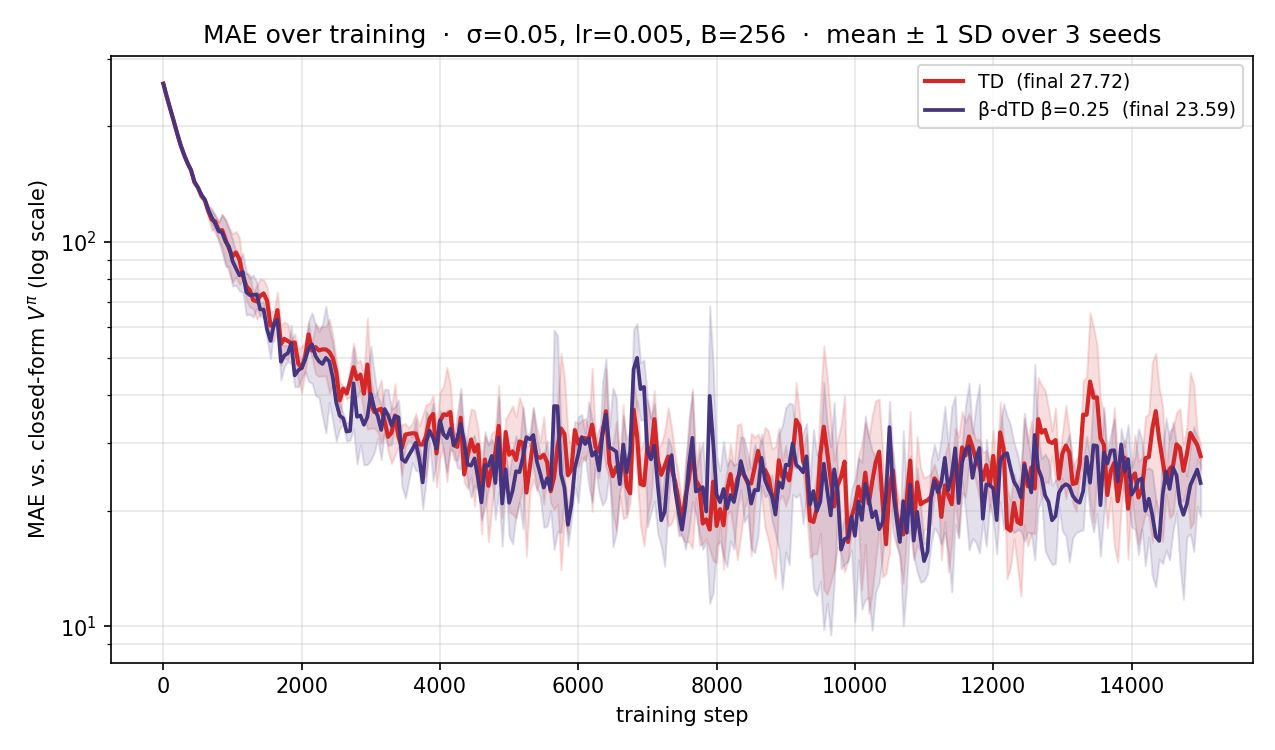
\includegraphics[width=0.6\textwidth]{media/MAE_over_time_dtd.jpeg}
    \caption{Evolution of MAE over training steps: $\beta$-dTD does not exhibit a faster rate of improvement than standard TD.}
    \label{fig:faster_rate}
\end{figure}







\section{Methodological Extensions \& Variance Reduction}
\label{sec:extensions}

\subsection{The \texorpdfstring{$K$}{K}-sample method}
To reduce the noise of the estimator in \cref{eq:noise}, we use the $K$-sample method. For each sampled wealth level $w_i$, we draw $K$ independent transitions to the next-state wealth, $w_{i,t+\Delta t}^{(1)}, \dots, w_{i,t+\Delta t}^{(K)}$, and average over them. This reduces the standard deviation of the estimator by a factor of $\sqrt{K}$, equivalently reducing its variance by a factor of $K$.

This has two drawbacks:
\begin{enumerate}
    \item \textbf{Financially unrealistic:} it requires sampling $K$ times from the conditional distribution $w_{t+\Delta t} \mid w_i$. In practice, one observes single trajectories of the asset without access to this distribution, so the method is only justified when a simulator or generative environment is available.
    \item \textbf{Higher computational cost:} both compute and memory grow by roughly a factor of $K$, which limits the size of $K$.
\end{enumerate}

\subsubsection{Results of the \texorpdfstring{$K$}{K}-sample method for pure dTD}
Our main empirical findings are that the use of the method helps pure dTD to no longer collapse to a constant function in the infinite-horizon setting. Using $K=10{,}000$, we obtain the approximation of the value function presented in \cref{fig:k10000dTD-infinite-horizon} after $12{,}000$ gradient steps.

This result indicates that sufficiently strong conditional averaging seems to prevent the constant-collapse failure mode. However, it does not establish convergence superior to that of TD and requires a prohibitively large number of simulated transitions over several seeds.

\subsubsection{Results of the K-sample method for \texorpdfstring{$\beta$}{beta}-dTD}

Several experiments were conducted to test the method on the loss of $\beta$-dTD in the infinite horizon setting. Our first empirical findings were that the use of small values of $K$ does not consistently help $\beta$-dTD achieve better results. Here, $K=32$ samples were used in each transition. As demonstrated by the results in \cref{tab:beta_dtd_results}, a significant performance improvement is observed at $\beta=0.9$, where the optimization objective is heavily dominated by the dTD component. However, as evidenced by the results using higher values of $K$ in subsequent sections, we conclude that 32 samples are insufficient to adequately suppress the large variance of the dTD estimator.

\subsection{Finite Horizon Merton problems}
Our next methodological extension consists of studying the finite horizon formulation of \cref{Merton-cost}. At some $T<\infty$, a terminal condition is imposed. Although we do not explicitly list it here, the value function still admits a known closed-form expression, which now also depends on time. This additional temporal structure may regularize the learning problem in the sense that the terminal condition anchors the value function at $t=T$, while the critic must learn a coherent evolution of the value function in both time and wealth. This differs from the infinite-horizon setting, where a constant function can more easily emerge as a stationary solution of the dTD problem.
%Note that the absolute MAEs here are not comparable to the infinite-horizon ones: with $T=1$ and no bequest, the target value function has mean magnitude $\approx 7$ over our grid versus $\approx 230$ infinite-horizon (a $\sim 30\times$ gap from the small $\kappa^*$). The much smaller MAEs below thus mostly reflect this rescaling, though the finite-horizon fits are also modestly better in relative terms ($\sim 1\text{--}2\%$ vs.\ $\sim 5\text{--}15\%$).


We evaluate and compare the empirical performance of standard TD and $\beta$-dTD in the finite-horizon Merton setting across several learning rates, batch sizes, random seeds and under two distinct volatility regimes. This experiment was executed using a single sample ($K = 1$) per wealth level within each mini-batch.


\begin{table}[t]
    \centering
    \caption{Best finite-horizon performance of TD and $\beta$-dTD (best MAE over training, mean $\pm$ std over three random seeds).}
    \label{tab:finite_horizon_hpo}
    \small
    \begin{tabular}{cccc}
        \toprule
        $\sigma$
        & Best TD MAE
        & Best $\beta$-dTD MAE
        & Best $\beta$ \\
        \midrule
        $0.05$ & $0.110 \pm 0.030$ & $\mathbf{0.082 \pm 0.015}$ & $0.75$  \\
        $0.20$ & $0.111 \pm 0.010$ & $\mathbf{0.100 \pm 0.009}$ & $0.25$ \\
        \bottomrule
    \end{tabular}
\end{table}

\Cref{tab:finite_horizon_hpo} reports the best configuration for each method, averaged over three seeds. At both volatility levels, $\beta$-dTD attains a lower MAE than standard TD. Crucially, this performance is achieved even with $K=1$, omitting the multi-sample conditional averaging that was strictly required to anchor convergence in the infinite-horizon regime. The advantage is clearest at low volatility ($\sigma=0.05$), where the search selects a high differential weight $\beta=0.75$: the dTD term then contributes most of the loss and still produces a stable and accurate critic. However, the gains are modest relative to seed-to-seed spread, and the error bars partially overlap, especially at $\sigma=0.20$, so we read the effect as consistent in sign rather than large in magnitude.

As volatility increases to $\sigma=0.20$, the selected weight falls to $\beta=0.25$ and the improvement over TD shrinks. This is consistent with the infinite-horizon experiments: the terminal condition and explicit time dependence of the finite-horizon value function regularize the differential term and keep it from collapsing, but they do not remove its underlying sensitivity to diffusion. At higher noise, the network therefore leans more towards the TD component, settling closer to the pure-TD baseline. The complete sweep of the hyperparameter is shown in \cref{fig:finite-horizon-sigma-comparison} in the appendix.

\subsection{Other approaches considered}
Additionally, we tested a method to bias the drift estimator towards zero. However, this did not yield the desired positive effects.

% We also attempted to introduce a scheduled beta progression to harness the faster convergence of $\beta$-dTD in the initial stages and then fall back to standard TD learning to explore the solution space. This was also unsuccessful.

\section{Conclusion \& Future Outlook}
\label{sec:conclusion}

We evaluated the differential temporal difference (dTD) framework of \citet{settai2025} beyond the drift-dominated control tasks for which it was designed, asking whether its continuous-time prior survives the noise-dominated regime of financial markets. Three conclusions emerge.

First, we replicated the Brax benchmarks: the hybrid $\beta$-dTD scheme attains faster early policy improvement than standard TD while converging to the same asymptotic return, with non-negligible tuned $\beta$ across all four environments, whereas naive-dTD offers no advantage.

Second, extending the evaluation to the genuinely SDE-driven Merton problem exposed a failure mode the deterministic benchmarks could not reveal. The drift estimator in the dTD residual is asymptotically unbiased but carries noise of order $\|\sigma\,\nabla V\|/\sqrt{\Delta t}$, which diverges as $\Delta t \to 0$ and grows with $\sigma$; in high-diffusion regimes it drives the critic to the spurious solution $\nabla V \to 0$, collapsing the value function to a constant. This collapse persists even when the network is initialized at the analytical optimum, confirming that the pathology is a property of the loss, not of optimization.

Third, we examine two remedies. The $K$-sample estimator prevents collapse in the infinite-horizon setting, but only at large $K$, at a roughly $K$-fold cost, and presupposes a simulator that can be requeried from the same state---unrealistic for observed financial data. The finite-horizon formulation is more promising: its terminal condition and explicit time dependence anchor the value function, letting $\beta$-dTD beat standard TD at both volatilities tested, with the largest gain at low volatility. However, the optimal $\beta$ decreases as volatility increases, showing that diffusion noise still erodes the benefit of the continuous-time term.

Taken together, these findings temper the promise of HJB-based reinforcement learning in finance: the prior that makes dTD attractive in drift-governed systems becomes a liability under heavy diffusion. Several directions follow: a \emph{multi-asset} Merton problem, to test whether higher state dimension helps the prior; a full \emph{actor-critic} formulation (the policy was fixed at its optimum here) to test dTD end-to-end; variance-reduction schemes beyond $K$-sampling that avoid resampling from the same state; and a \emph{dynamic} $\beta$ that exploits early dTD acceleration and anneals toward TD as the critic stabilizes.

\newpage
\appendix


\section{Supplementary material}{\label{supp-mat}}

\begin{figure}[h]
    \centering
    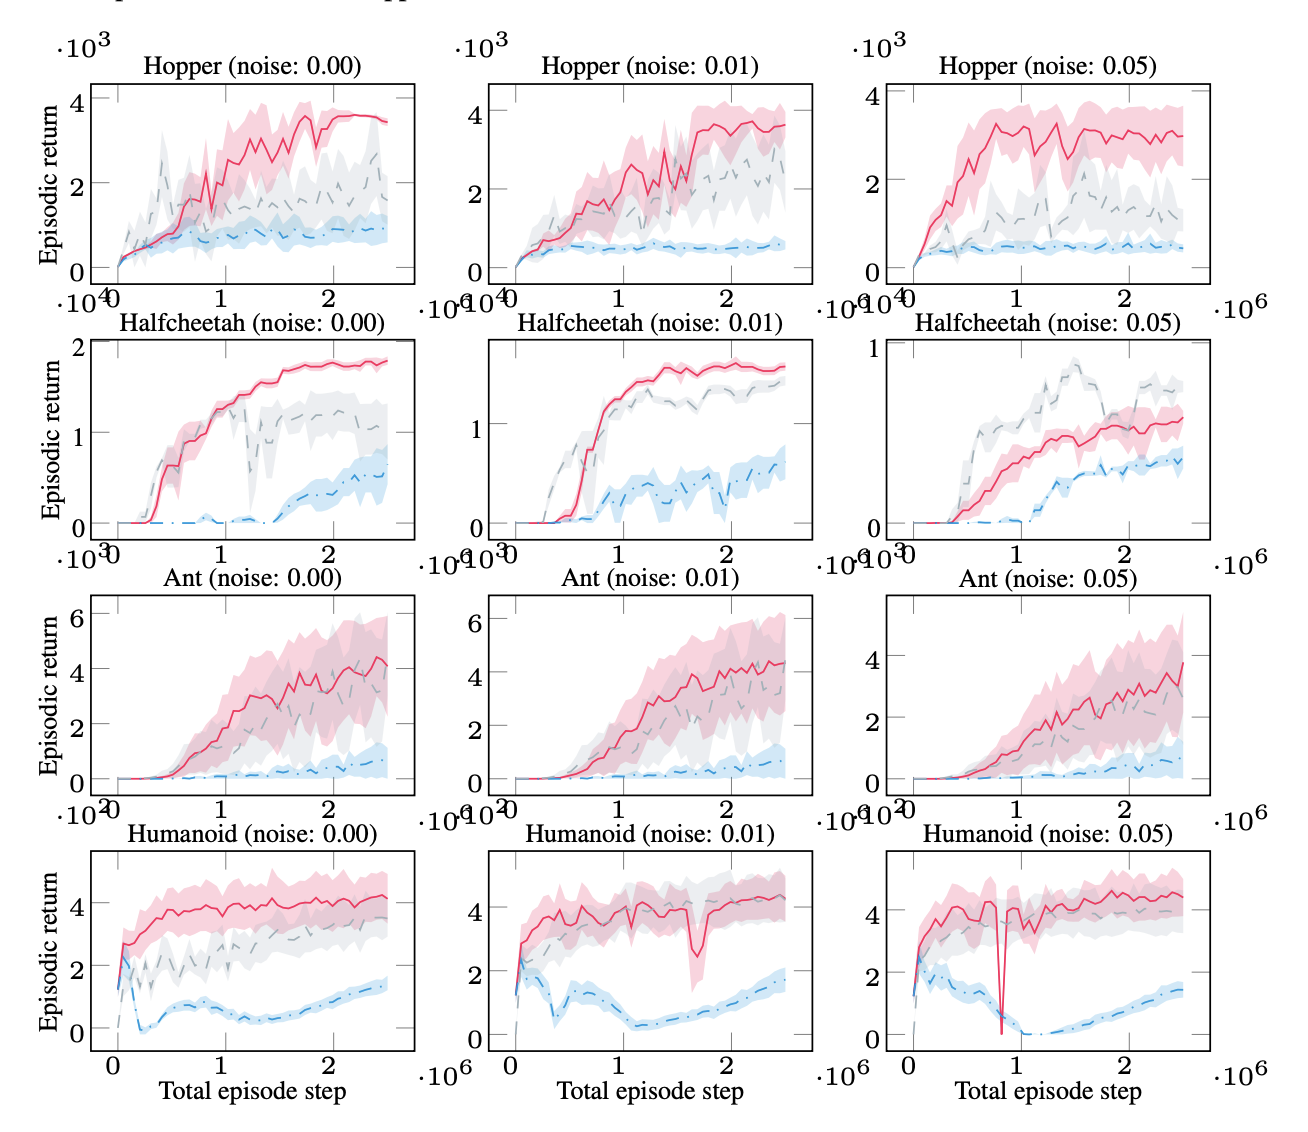
\includegraphics[width=0.85\textwidth,height=0.40\textheight,keepaspectratio]{media/SettaiResults.png}
    \caption{Original baseline results of \citet{settai2025}, reproduced for comparison with our replication in \cref{fig:replication_comparison}. $\beta$-dTD in red, TD in grey, $\beta$-naive-dTD in blue.}
    \label{fig:paper_res}
\end{figure}

\begin{figure}[h]
    \centering
    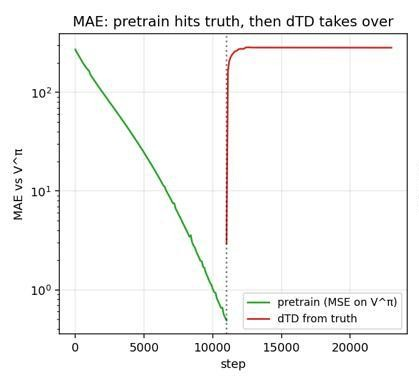
\includegraphics[width=0.6\textwidth]{media/pretrained_dtd.jpeg}
    \caption{MAE for learned value function starting from a pre-trained network. As soon as TD loss is used, the error starts to grow.}
    \label{fig:pretrained}
\end{figure}

\begin{figure}[p]
    \centering
    \begin{subfigure}[b]{\textwidth}
        \centering
        
\includegraphics[width=0.85\textwidth,height=0.40\textheight,keepaspectratio]{{media/grid_dtd_high_noise.jpeg}}
        \caption{Hyperparameter performance for $\beta$-dTD with \textbf{high} noise}
        \label{fig:high_noise}
    \end{subfigure}

    \vspace{0.3cm}

    \begin{subfigure}[b]{\textwidth}
        \centering
        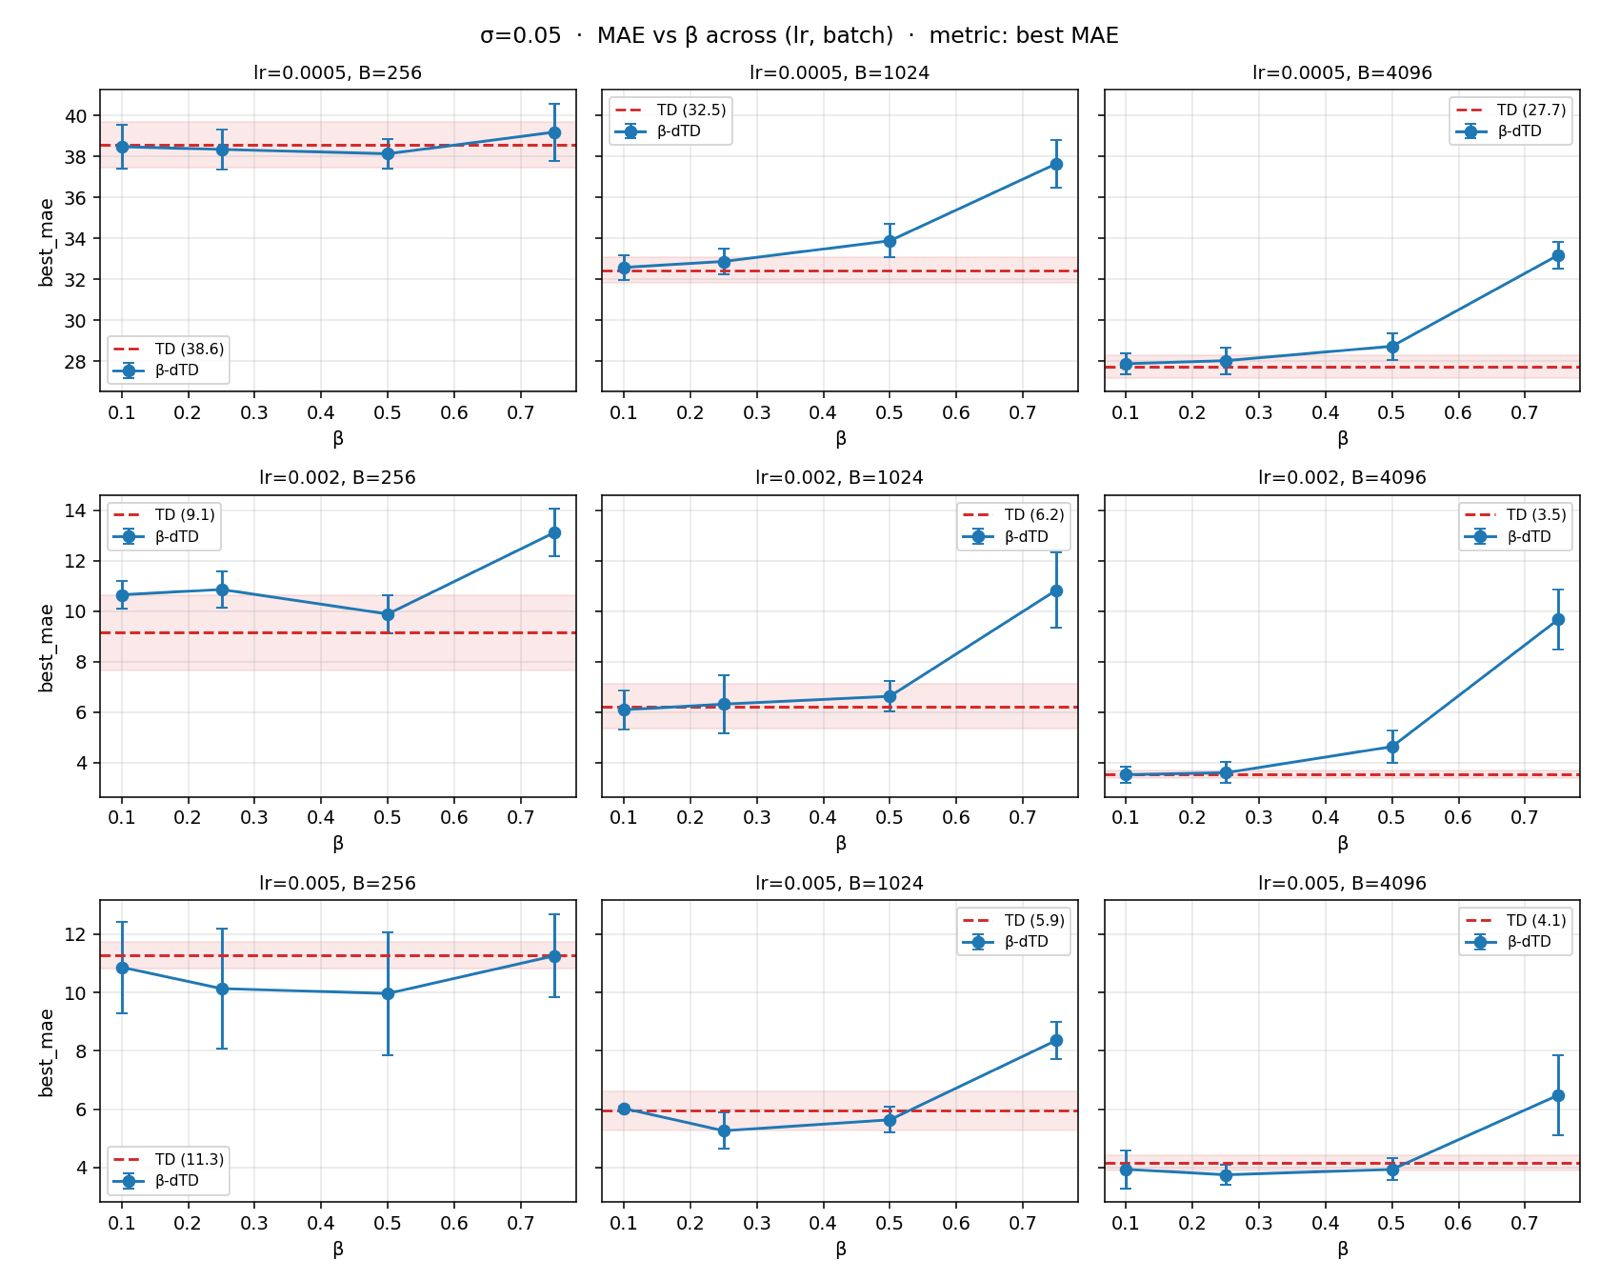
\includegraphics[width=0.85\textwidth,height=0.40\textheight,keepaspectratio]{media/grid_dtd_low_noise.jpeg}
        \caption{Hyperparameter performance for $\beta$-dTD with \textbf{low} noise}
        \label{fig:low_noise}
    \end{subfigure}

    \caption{$\beta$-dTD performance in the infinite Merton problem for different hyperparameters configuration.}
    \label{fig:low_vs_high_noise}
\end{figure}


\begin{figure}[h]
    \centering
    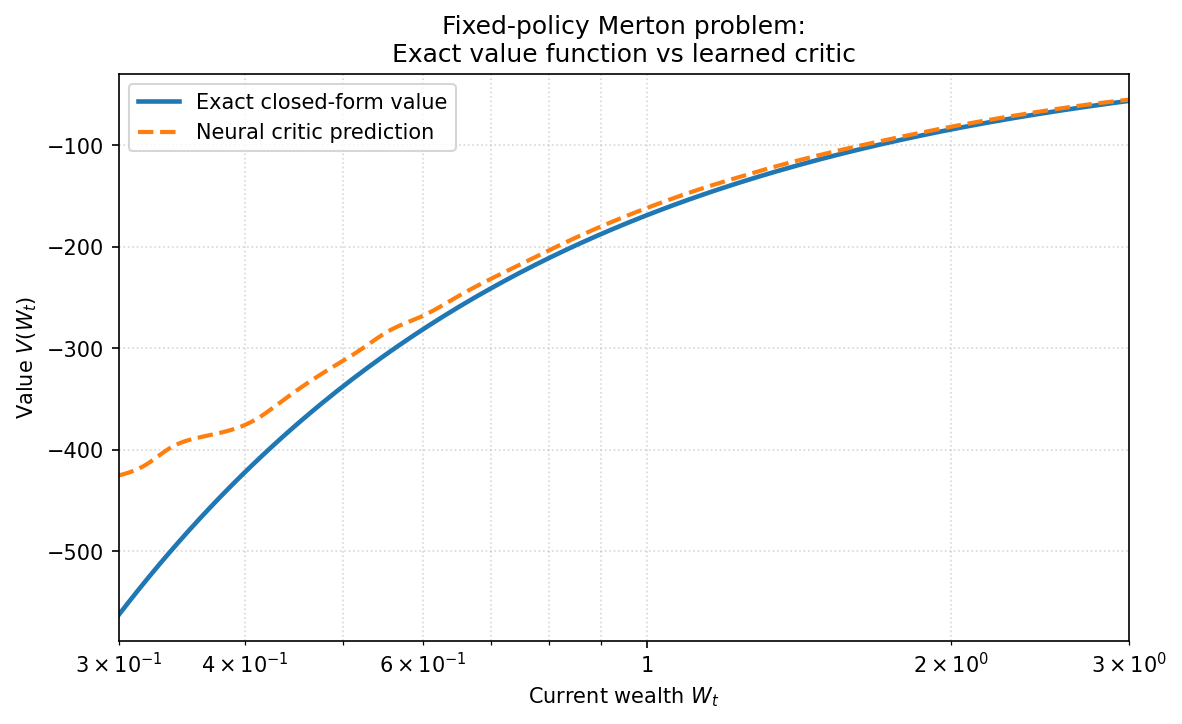
\includegraphics[width=0.7\textwidth]{media/K_10000.png}
    \caption{Value function approximation learned using $K=10{,}000$ samples with pure dTD in the infinite-horizon setup. Batch size 512, $12{,}000$ gradient steps, $\Delta t=1/252$, $\sigma=0.20$.}
    \label{fig:k10000dTD-infinite-horizon}
\end{figure}

\begin{table}[htbp]
\centering
\caption{Infinite-horizon MAE (best over training, mean $\pm$ std over 3 seeds) across mixture weights $\beta$. Batch size 256, $\sigma=0.05$, $\Delta t=1/252$. The first column ($\beta$-dTD) is the classic $K=1$ loss; the second uses $K=32$ conditional samples per transition.}
\label{tab:beta_dtd_results}
\begin{tabular}{ccc}
\toprule
\textbf{\boldmath$\beta$} & \textbf{\boldmath$\beta$-dTD $(K=1)$} & \textbf{\boldmath$\beta$-dTD-mean $(K=32)$} \\
\midrule
0.25 & $10.1 \pm 2.0$ & $10.5 \pm 1.5$ \\
0.50 & $10.0 \pm 2.1$ & $10.7 \pm 0.6$ \\
0.75 & $11.2 \pm 1.4$ & $10.9 \pm 1.0$ \\
0.90 & $21.4 \pm 2.9$ & $\mathbf{10.3 \pm 1.1}$ \\
\bottomrule
\end{tabular}
\end{table}

\begin{figure}[p]
    \centering
    \begin{subfigure}[b]{\textwidth}
        \centering
        
\includegraphics[width=0.85\textwidth,height=0.40\textheight,keepaspectratio]{{media/sigma0.05_best_mae_vs_beta.png}}
        \caption{Hyperparameter performance for $\beta$-dTD with \textbf{low} noise}
        \label{fig:finite-horizon-low-noise}
    \end{subfigure}

    \vspace{0.3cm}

    \begin{subfigure}[b]{\textwidth}
        \centering
        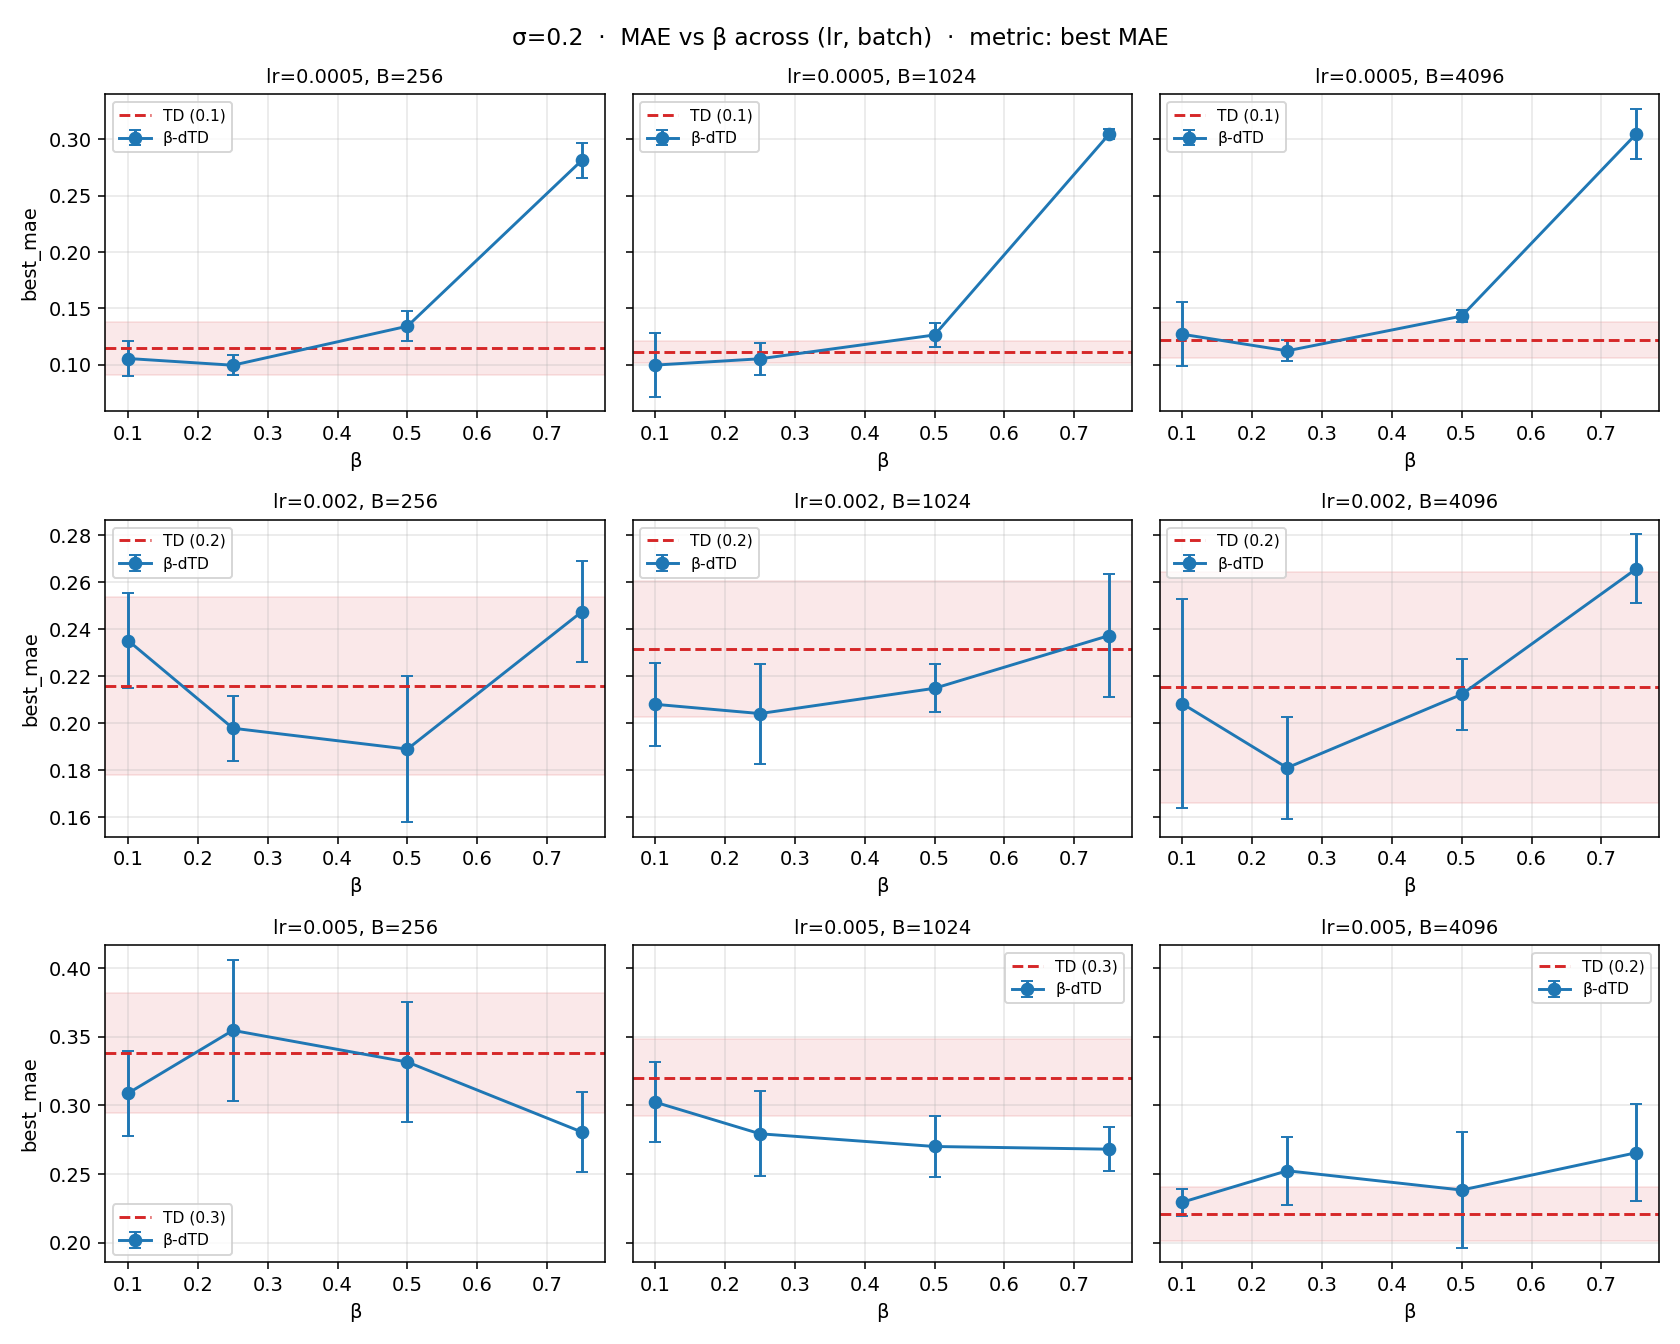
\includegraphics[width=0.85\textwidth,height=0.40\textheight,keepaspectratio]{media/sigma0.2_best_mae_vs_beta.png}
        \caption{Hyperparameter performance for $\beta$-dTD with \textbf{high} noise}
        \label{fig:finite-horizon-high-noise}
    \end{subfigure}

    \caption{$\beta$-dTD performance in the finite horizon Merton problem for different hyperparameters configuration.}
    \label{fig:finite-horizon-sigma-comparison}
\end{figure}



\clearpage
\bibliographystyle{plainnat}
\bibliography{references}


\end{document}
